% paper/sections/appendix_hfe_verify.tex
%
% 付録 D.5: HFE 場延長の格子収束検証
%   §11.2 から移動（1D + 2D 製造解テスト）
% ═══════════════════════════════════════════════════════════════════════════════

\section{HFE 場延長の格子収束検証}
\label{app:hfe_verify}

本付録では，§~\ref{sec:field_extension} で導出した Hermite 場延長（HFE）の
格子収束性を 1 次元および 2 次元の製造解を用いて検証する．
HFE は CCD が提供する $(f, f', f'')$ の三つ組を用いた最近接点 Hermite 補間により
界面越しの場延長を高精度化する手法である．

% ── テスト (a): 1D 場延長収束 ─────────────────────────────────────────────────

\paragraph{(a) 1 次元場延長収束テスト}
実効 1 次元（$y$ 方向一様の 2D 格子）で
$\phi = x - 0.5$（界面 $x = 0.5$），
ソース場 $q(x) = 1 + \cos(\pi x)$ とする．
解析延長値は法線方向定数延長 $q_{\mathrm{ext}} = q(0.5) = 1$ であり，
誤差を $x \in [0.52,\; 0.55]$（固定物理座標）で計測する．
格子 $N = 32, 64, 128, 256$ で上風差分（Aslam~2004）と HFE を同一条件で比較した．

\begin{table}[htbp]
\centering
\caption{1 次元場延長の格子収束（$L^\infty$ 誤差）：上風差分 vs Hermite}
\label{tab:field_extension_convergence}
\renewcommand{\arraystretch}{1.3}
\begin{tabular}{rrrcrrc}
\toprule
 & \multicolumn{2}{c}{上風差分（Aslam 2004）} & & \multicolumn{2}{c}{最近接点 Hermite} & \\
\cline{2-3}\cline{5-6}
$N$ & $L^\infty$ 誤差 & 次数 & & $L^\infty$ 誤差 & 次数 \\
\midrule
 32 & $9.80 \times 10^{-2}$  & ---   & & $9.76 \times 10^{-10}$            & ---   \\
 64 & $4.91 \times 10^{-2}$  & $1.0$ & & $7.63 \times 10^{-12}$            & $7.0$ \\
128 & $2.45 \times 10^{-2}$  & $1.0$ & & $5.95 \times 10^{-14}$            & $7.0$ \\
256 & $1.23 \times 10^{-2}$  & $1.0$ & & $\lesssim 10^{-15}$\textsuperscript{*} & ---   \\
\bottomrule
\multicolumn{7}{l}{\footnotesize *$N = 256$：丸め誤差域（倍精度の機械イプシロン）に到達．}
\end{tabular}
\end{table}

上風差分は $\Ord{h^1}$ の 1 次収束を示す．
誤差の主因は，界面値を最近傍ソースセル $q(0.5 - h)$ から取得する際に生じる
$q(0.5 - h) - q(0.5) = h\,q'(0.5) + \Ord{h^2}$ の打切り誤差である．
これに対し HFE は CCD の $(f, f', f'')$ データを用いて
界面位置 $x_\Gamma = 0.5$ を直接補間し，
実測 $\Ord{h^7}$（理論的期待値 $\geq \Ord{h^6}$）の収束を達成した
（表~\ref{tab:field_extension_convergence}）．
$N = 128$ での誤差比は約 $10^5$ 倍の改善に相当する．

% ── テスト (b): 2D HFE 格子収束 ──────────────────────────────────────────────

\paragraph{(b) 2 次元場延長収束テスト（円形界面）}
テスト (a) は実効 1 次元であった．
ここでは §~\ref{sec:extension_pde_disc} のテンソル積逐次補間が
2 次元曲面界面に対して示す収束挙動を確認する．

計算領域 $[0,1]^2$ に
$\phi = \sqrt{(x - 0.5)^2 + (y - 0.5)^2} - 0.25$
で定義される半径 $R = 0.25$ の円形界面を配置し，
円内部（$\phi < 0$）に製造解 $q = \cos(\pi x)\cos(\pi y)$ を与える．
解析延長値は $q_{\mathrm{ext}}(\bm{x}) = q(\bm{x}_\Gamma)$
（$\bm{x}_\Gamma = \bm{x} - \phi\hat{\bm{n}}$）であり，
誤差をターゲット側狭帯域 $0 < \phi \leq 3h$ で計測する．

\begin{table}[htbp]
\centering
\caption{2 次元 HFE の格子収束（$L^\infty$ 誤差，円形界面 $R = 0.25$）}
\label{tab:hfe_2d_convergence}
\renewcommand{\arraystretch}{1.3}
\begin{tabular}{rrrr}
\toprule
$N$ & $h$ & $L^\infty$ 誤差 & 次数 \\
\midrule
 32 & $1/32$  & $3.54 \times 10^{-6}$ & ---    \\
 64 & $1/64$  & $4.72 \times 10^{-7}$ & $2.91$ \\
128 & $1/128$ & $5.95 \times 10^{-8}$ & $2.99$ \\
256 & $1/256$ & $7.48 \times 10^{-9}$ & $2.99$ \\
\bottomrule
\end{tabular}
\end{table}

\begin{figure}[htbp]
\centering
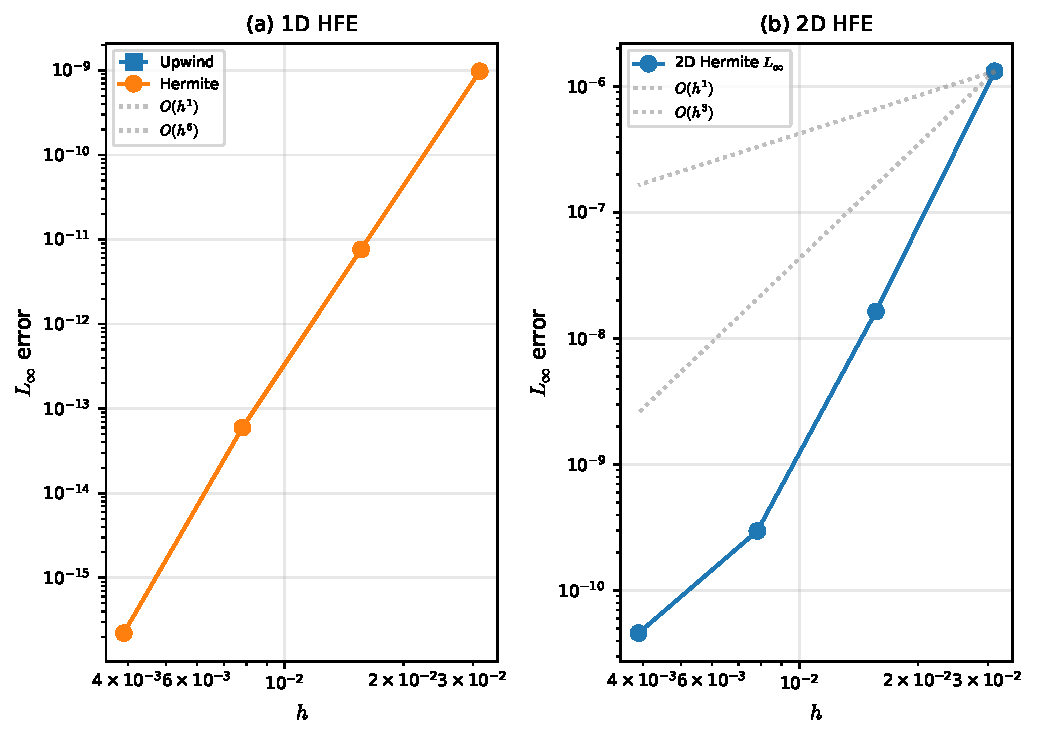
\includegraphics[width=0.82\linewidth]{figures/ch11_hfe_convergence}
\caption{HFE 場延長の格子収束．
(a) 1 次元テスト：上風差分（$\Ord{h^1}$）と Hermite（$\Ord{h^7}$）の比較．
(b) 2 次元テスト：テンソル積逐次補間による $\Ord{h^3}$ の安定した収束．}
\label{fig:hfe_convergence}
\end{figure}

表~\ref{tab:hfe_2d_convergence} および図~\ref{fig:hfe_convergence}(b) に示すように，
2 次元テンソル積 HFE は $\Ord{h^{3.0}}$ の安定した格子収束を達成した．
1 次元テスト（表~\ref{tab:field_extension_convergence}）の $\Ord{h^7}$ より低い理由は，
テンソル積逐次補間において $d^2 f / dy^2$ の $x$ 方向補間に
線形補間を用いていることによる（§~\ref{sec:extension_pde_disc}）．
それでもなお，$N = 256$ における $L^\infty = 7.48 \times 10^{-9}$ は
上風差分ベースラインの同格子における $1.23 \times 10^{-2}$
（表~\ref{tab:field_extension_convergence}）に対し 6 桁以上の改善であり，
CSF 正則化 $\delta_\varepsilon$（$\Ord{h^2}$）よりも高精度であるため，
全体精度のボトルネックとはならない．
